\documentclass{article}

% Set page size and margins
% Replace `letterpaper' with`a4paper' for UK/EU standard size
\usepackage[letterpaper,top=2cm,bottom=2cm,left=3cm,right=3cm,marginparwidth=1.75cm]{geometry}

% Useful packages
\usepackage{amsmath}
\usepackage{graphicx}
\usepackage[colorlinks=true, allcolors=blue]{hyperref}
\usepackage{float}
\usepackage{booktabs}

\title{\textit{Jeopardy!} High-Win Binary Classification}
\author{Thomas Mondry}

\begin{document}
	\maketitle
	
	\section{Abstract}
	
	Using complete \textit{Jeopardy!} game data from the \textit{J! Archive} site, I build models to predict whether or not a player will win more than three games, given any available information from their first game. Additionally, I identify quantifiable attributes of a player's first game which are useful in making such predictions.
	
	\section{Introduction}
	
	Jeopardy! is one of the longest-running and most beloved American game shows. Groups of three players compete for cash prizes by answering trivia questions and placing wagers. Winning contestants then compete in the next game, with no upper limit to how much a player may win or how many games they can play. Successful contestants (like Ken Jennings, James Holzhauer, and Matt Amodio) may garner substantial media attention, TV hosting opportunities, and positions on other game	shows. However, very few contestants are able to dominate games so completely that they win more than three games in a row. Contestants who win five or more games are automatically eligible for one of 	fifteen spots in the Tournament of Champions, with four-game winners also often invited to fill the remaining positions. In this project, I attempt to build a model to identify these strong players early, using data from only their first game played. I examine two research questions: first, I build a full model of whether or not a player will win many games, using all available numeric information, with predictive accuracy as the only goal. Second, I identify which quantifiable attributes of a player's first game are most useful in making these predictions.
	
	\section{Data}
	
	I use data from all televised \textit{Jeopardy!} games over the 20-year period from April 19, 2002, to April 21, 2022, except games from special tournaments -- Tournaments of Champions, college, teen, teachers, kids, celebrity, or other special tournaments. This totals 3764 games. All of the games included in the data have in common the attribute that the winner of one game appears again in the next game, and does so until they lose a game. This allows me to calculate the dependent variable from the data.
	
	I acquire the data through web scraping with \texttt{rvest} and pull essentially all information about a game. The output from this process is a list of three objects:
	
	\begin{enumerate}
		
		\item \textbf{Clue-level information:} A list of length equal to the number of games in the data; each element is a data frame with 60 rows corresponding to the 30 Jeopardy round and 30 Double Jeopardy round clues, and each row contains information about the round, category, dollar value, and content of the clue; the order in which that clue came up in the game; whether or not that clue is a Daily Double and, if so, the amount of the wager; and each player's performance on that clue (correct, incorrect or no answer)
		
		\item \textbf{Player-level information:} A list of length equal to the number of games in the data; each element is a data frame with 3 rows corresponding to the 3 players in the game, and each row contains information about the player's name, occupation, scores after the Jeopardy and Double Jeopardy rounds, Final Jeopardy wager, performance on Final Jeopardy (correct or incorrect), final score, and Coryat score (a metric which neither rewards nor punishes aggressive or conservative betting behavior, and which disregards Final Jeopardy)
		
		\item \textbf{Game-level information:} A data frame of row length equal to the number of games in the data; each row contains some basic information about the game as well as the Final Jeopardy category and clue, which do not have a natural place elsewhere but may be useful
		
	\end{enumerate}

	After creating this general data object, I use it to create a tabular dataset which is tailored specifically to my research question. I calculate each winner's ultimate win count and associate this information with their first game; I then discard other data from games in which a player does not achieve their first win, as this data is outside the scope of my research question. This leaves 1918 of the original 3764 games, and 1918 unique winners.
	
	To determine the threshold for how many wins should be considered "high-win", I examine the frequency of the win count variable and find that setting the threshold at >3 games results in 10\% of players being classified as high-winners; this seems appropriate.
	
	\begin{figure}[H]
		\centering
		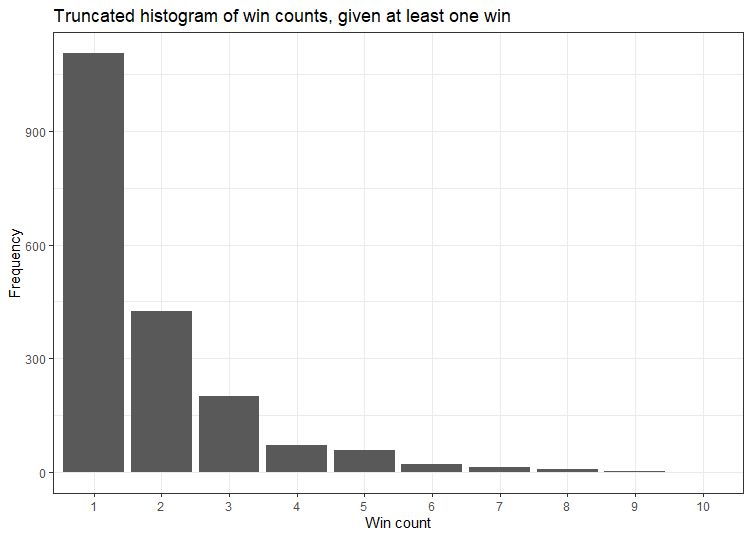
\includegraphics[width=\textwidth]{win_count_hist.png}
		\caption{Histogram of a player's win count, given at least one win (truncated at 10 wins for legibility)}
	\end{figure}
	
	I create numerical features and fill them for each observation, as shown in Table 2. There is no missing data from this process, and the full dataset used for modeling has 31 numeric features.
	
		\begin{table}[H]
		\centering
		\caption{All predictor variables\\}
			\begin{tabular}{l}
				\hline
				Returning champion's win count \\
				Each player's score after the Jeopardy round \\
				Each player's score after the Double Jeopardy round \\
				Each player's Coryat score \\
				Each player's Final Jeopardy wager \\
				Each player's final score \\
				For each player, a binary indicator of whether they answered Final Jeopardy correctly \\
				Each player's number of correct answers \\
				Each player's number of incorrect answers \\
				Each player's longest streak of correct answers \\
				For each player, the ordered index of the first clue answered correctly
			\end{tabular}
	\end{table}
	
	\section{Methods}
	
	First, I attempt to model the outcome directly, using all available numeric features. I use an 80\%/20\% test/train split on the 1918 available observations to train few different ML algorithms, tuning model hyperparameters using 5-fold cross-validation.
	
	Given that it appears it won't be possible to meaningfully model the outcome using the available data, I will now move toward examining my secondary research question, which is to identify some features which provide the most useful information toward predicting the outcome. Since this question pertains to parameter estimation rather than prediction, I will part with the test-train split and build many logit sub-models which contain only a few features, starting with the models which contain only one feature. I will use my intuition and the results of the simplest models to select variables for inclusion which are less likely to be highly intercorrelated. Most of the features in the full model are very highly correlated with each other, but this is not a concern for answering my first research question, since prediction is my only concern. When I begin to consider my second research question, it will be necessary to decrease intercorrelation as much as possible.
	
	\section{Findings}
	
	To get a good start on this, I trained models using 4 different ML algorithms, using area under the ROC curve as a model evaluation metric. The preliminary results indicate to me that this research question is probably not worth pursuing, since the area under the ROC curve is not far over the expected "random guessing" outcome of 0.5:
	
	\begin{table}[H]
		\centering
		\caption{Model hyperparameters and results\\}
			\begin{tabular}{l|r|r|r|r|r|r|r}
				\hline
				Algorithm & Area under ROC curve & Std. error & Model hyperparameters\\
				\hline
				Penalized logit (LASSO) & 0.51933 & 0.01339 & $\lambda$ = 0.009103\\
				\hline
				Neural network & 0.54143 & 0.02214 & $\lambda$ = 1, 5 hidden units\\
				\hline
				k-Nearest neigbors & 0.51776 & 0.02231 & k = 2\\
				\hline
				Support vector machine & 0.51782 & 0.01525 & cost = 1024, $\sigma$ = 0.5\\
				\hline
			\end{tabular}
	\end{table}

	Therefore, as I explained in the section above, I will now focus on my second research question.
	
	\section{References}
	
	I'm having issues with LaTeX, so I wasn't able to get the bibliography to appear here; it is complete and saved in the PS11 directory on my repo.
	
	
\end{document}